\chapter{Compositions of Integers}

Compositions are the first family of objects we count systematically with generating series.
They are simple enough that everything can be checked by hand, yet they already show the
whole method: describe the set as a Cartesian product or sequence, apply the sum, product and
string lemmas, then extract coefficients.

\section{Compositions}

\begin{definition}[Composition]
A \emph{composition} of a non-negative integer $n$ with $k$ parts is a $k$-tuple
$(c_1, \dots, c_k)$ of \emph{positive} integers with $c_1 + \cdots + c_k = n$. The $c_i$ are
the \emph{parts}. The empty tuple is the unique composition of $0$ (with $0$ parts).
\end{definition}

Order matters: $(1,2)$ and $(2,1)$ are different compositions of $3$. The compositions of $4$ are
\[
(4),\ (3,1),\ (1,3),\ (2,2),\ (2,1,1),\ (1,2,1),\ (1,1,2),\ (1,1,1,1),
\]
eight in total.

\begin{theorem}
For $n, k \ge 1$, the number of compositions of $n$ with $k$ parts is $\binom{n-1}{k-1}$.
\end{theorem}
\begin{proof}
Let $\N_{\ge1} = \{1, 2, 3, \dots\}$ with weight $w(c) = c$, so
$\Phi_{\N_{\ge1}}(x) = x + x^2 + \cdots = \frac{x}{1-x}$. Compositions with $k$ parts are the
elements of $\N_{\ge1}^k$ with weight the sum of the parts, so by the product lemma their
generating series is $\left(\frac{x}{1-x}\right)^k$. Then
\[
\coef{n}\frac{x^k}{(1-x)^k} = \coef{n-k}\frac{1}{(1-x)^k} = \binom{n-k+k-1}{k-1} = \binom{n-1}{k-1}.
\]
\end{proof}

\begin{aside}
A bijective proof: write $n$ as a row of $n$ dots. A composition with $k$ parts corresponds to
choosing $k-1$ of the $n-1$ gaps between consecutive dots to cut. For example
$\bullet\bullet\,|\,\bullet\,|\,\bullet\bullet\bullet$ is $(2,1,3)$.
\end{aside}

Here are all eight compositions of $4$ drawn this way; each of the $3$ gaps is either cut or
not, which already shows there are $2^{3}$ of them (see the next theorem).
\begin{center}
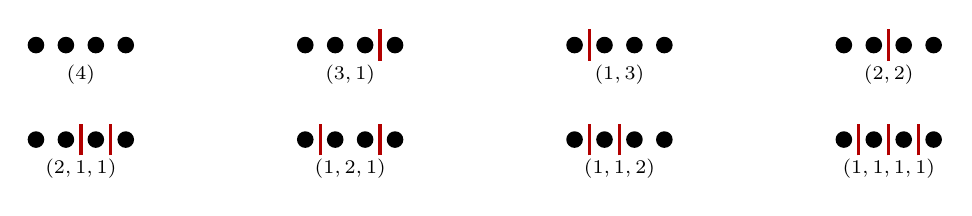
\begin{tikzpicture}[x=0.38cm,y=0.5cm]
  \foreach \cuts/\lab [count=\r from 0] in {{}/{(4)}, {3}/{(3,1)}, {1}/{(1,3)}, {2}/{(2,2)},
       {2,3}/{(2,1,1)}, {1,3}/{(1,2,1)}, {1,2}/{(1,1,2)}, {1,2,3}/{(1,1,1,1)}} {
    \pgfmathsetmacro{\xo}{mod(\r,4)*9}
    \pgfmathsetmacro{\yo}{-int(\r/4)*2.4}
    \begin{scope}[shift={(\xo,\yo)}]
      \foreach \d in {1,...,4} { \fill (\d,0) circle (3pt); }
      \foreach \c in \cuts { \draw[very thick,red!70!black] (\c+0.5,-0.4) -- (\c+0.5,0.4); }
      \node[font=\scriptsize] at (2.5,-0.75) {$\lab$};
    \end{scope}
  }
\end{tikzpicture}
\end{center}

\begin{theorem}
For $n \ge 1$ the total number of compositions of $n$ is $2^{n-1}$.
\end{theorem}
\begin{proof}
The set of all compositions is $\N_{\ge1}^* = \bigcup_{k\ge0}\N_{\ge1}^k$, and $\N_{\ge1}$ has no
element of weight $0$, so by the string lemma
\[
\Phi(x) = \frac{1}{1 - \frac{x}{1-x}} = \frac{1-x}{1-2x} = \frac{1}{1-2x} - \frac{x}{1-2x}.
\]
Hence $\coef{n}\Phi = 2^n - 2^{n-1} = 2^{n-1}$ for $n \ge 1$ (and $\coef{0}\Phi = 1$).
\end{proof}

\section{Compositions with restricted parts}

The general recipe: if the parts are required to lie in a set $P \subseteq \N_{\ge1}$, then
\[
\text{compositions with $k$ parts in $P$:}\quad \Phi_P(x)^k,
\qquad \text{all compositions with parts in $P$:}\quad \frac{1}{1 - \Phi_P(x)}.
\]
If each part has its own restriction, $c_i \in P_i$, the product lemma gives
$\Phi_{P_1}(x)\cdots\Phi_{P_k}(x)$.

\begin{example}[Parts equal to $1$ or $2$]
$P = \{1,2\}$, $\Phi_P = x + x^2$, so the generating series is $\frac{1}{1 - x - x^2}$. If $c_n$
is the coefficient of $x^n$, then from $(1-x-x^2)\sum c_nx^n = 1$ we get $c_0 = 1$, $c_1 = 1$
and $c_n = c_{n-1} + c_{n-2}$ for $n \ge 2$: the Fibonacci numbers $1, 1, 2, 3, 5, 8, \dots$.
For $n = 3$ the compositions are $(1,1,1),(1,2),(2,1)$: three of them.
\end{example}

\begin{example}[Odd parts]
$P = \{1,3,5,\dots\}$, $\Phi_P = x + x^3 + x^5 + \cdots = \frac{x}{1-x^2}$, so the
generating series is
\[
\frac{1}{1 - \frac{x}{1-x^2}} = \frac{1-x^2}{1 - x - x^2}.
\]
With $a_n$ the coefficients, $a_n - a_{n-1} - a_{n-2}$ is $1$ for $n=0$, $-1$ for $n = 2$,
and $0$ otherwise. So $a_0 = 1$, $a_1 = 1$, $a_2 = 1+1-1 = 1$, $a_3 = 2$, $a_4 = 3$, $a_5 = 5$.
Check $n=4$: $(1,3),(3,1),(1,1,1,1)$, three compositions.
\end{example}

\begin{example}[Parts at least $2$]
$\Phi_P = \frac{x^2}{1-x}$, giving $\frac{1}{1 - \frac{x^2}{1-x}} = \frac{1-x}{1-x-x^2}$.
\end{example}

\begin{example}[Even parts, $k$ parts]
$\Phi_P = \frac{x^2}{1-x^2}$, so the series is $\frac{x^{2k}}{(1-x^2)^k}$. For $n = 2m$,
\[
\coef{2m}\frac{x^{2k}}{(1-x^2)^k} = \coef{2m-2k}\sum_{j\ge0}\binom{j+k-1}{k-1}x^{2j}
= \binom{m-k+k-1}{k-1} = \binom{m-1}{k-1},
\]
and the coefficient is $0$ for $n$ odd. This makes sense: halving every part is a bijection
with compositions of $m$ into $k$ parts.
\end{example}

\begin{example}[Bounded parts]
How many compositions of $10$ have $3$ parts, each at most $4$? The series is
$(x + x^2 + x^3 + x^4)^3 = x^3\left(\frac{1-x^4}{1-x}\right)^3$, so we need
\[
\coef{7}\frac{(1-x^4)^3}{(1-x)^3} = \coef{7}\frac{1 - 3x^4 + 3x^8 - x^{12}}{(1-x)^3}
= \binom{9}{2} - 3\binom{5}{2} = 36 - 30 = 6.
\]
Check directly: the part multisets are $\{4,4,2\}$ and $\{4,3,3\}$, each with $3$ orderings.
\end{example}

\begin{important}[Pitfall: the zero part]
Compositions have \emph{positive} parts. If a problem allows zero parts (e.g.\ non-negative
solutions of $t_1 + \cdots + t_k = n$), use $\frac{1}{1-x}$ for each part instead of
$\frac{x}{1-x}$; but then the string lemma does \emph{not} apply to ``any number of parts''
since $0$ has weight $0$.
\end{important}

\section{Subsets with restrictions}

Compositions encode many other objects through their \emph{gaps}.

\begin{theorem}
The number of $k$-subsets of $[n]$ containing no two consecutive integers is
$\binom{n-k+1}{k}$.
\end{theorem}
\begin{proof}
For a subset $\{a_1 < a_2 < \cdots < a_k\}$ of $[n]$, form the gap sequence
\[
(a_1,\ a_2 - a_1,\ a_3 - a_2,\ \dots,\ a_k - a_{k-1},\ n + 1 - a_k).
\]
This is a composition of $n+1$ with $k+1$ parts, and the map is a bijection (recover $a_i$ by
partial sums). The subset has no two consecutive elements iff the middle $k-1$ parts are all
at least $2$; the first and last parts are just at least $1$. So the generating series is
\[
\left(\frac{x}{1-x}\right)^2\left(\frac{x^2}{1-x}\right)^{k-1} = \frac{x^{2k}}{(1-x)^{k+1}},
\]
and the answer is $\coef{n+1}\frac{x^{2k}}{(1-x)^{k+1}} = \binom{n+1-2k+k}{k} = \binom{n-k+1}{k}$.
\end{proof}

\begin{example}
$n = 5$, $k = 2$: $\binom{4}{2} = 6$. The subsets are $\{1,3\},\{1,4\},\{1,5\},\{2,4\},\{2,5\},
\{3,5\}$.
\end{example}

For instance $\{2,4\} \subseteq [5]$ has gap sequence $(2,2,2)$, a composition of $6$ whose middle
part is at least $2$:
\begin{center}
\begin{tikzpicture}[x=1cm,>={Stealth}]
  \draw (0,0) -- (6,0);
  \foreach \i in {0,...,6} { \draw (\i,0.1) -- (\i,-0.1) node[below,font=\small] {$\i$}; }
  \foreach \i in {2,4} { \fill[blue!70!black] (\i,0) circle (3.5pt); }
  \draw[gray,dashed] (6,0.25) -- (6,-0.25);
  \foreach \a/\b/\l in {0/2/{a_1 = 2},2/4/{a_2 - a_1 = 2},4/6/{n+1-a_2 = 2}} {
    \draw[decorate,decoration={brace,amplitude=4pt}] (\a+0.05,0.25) -- (\b-0.05,0.25) node[midway,above=4pt,font=\scriptsize] {$\l$};
  }
\end{tikzpicture}
\end{center}

\section{Summary}
\begin{itemize}
  \item A composition of $n$ is an ordered tuple of positive integers summing to $n$.
  \item $k$ parts: $\left(\frac{x}{1-x}\right)^k$, giving $\binom{n-1}{k-1}$; any number of parts:
        $\frac{1-x}{1-2x}$, giving $2^{n-1}$ for $n \ge 1$.
  \item Parts in $P$: $\Phi_P^k$ or $1/(1 - \Phi_P)$. Parts in $\{1,2\}$ give Fibonacci numbers.
  \item Gap sequences turn subset problems into composition problems.
\end{itemize}
